\section{Introduction}
\label{Introduction}
The purpose of this mini project in Image Processing and Computer Vision, is to find a article which use a algorithm in some area of computer vision, and try to replicate their results. The chosen article is \parencite{Baoming2016}. The article is focused on optimizing a grey image edge detection algorithm which is based on grey correlation analysis. The optimization is based in making the thresholding of the edge detection adaptive. The goal of the improved algorithm is to get a end result with fewer falls positive edge detected, and better continuity in the detected edges. \autoref{fig:Sammenligning} is a figure from \parencite{Baoming2016} which shows the result using the optimized algorithm, compared to the original grey correlation analysis algorithm. On \autoref{fig:Sammenligning} the image in the bottom right corner is the result from the improved algorithm, while the other images is a result of different thresholds and operators.

\begin{figure}[H]
	\centering
	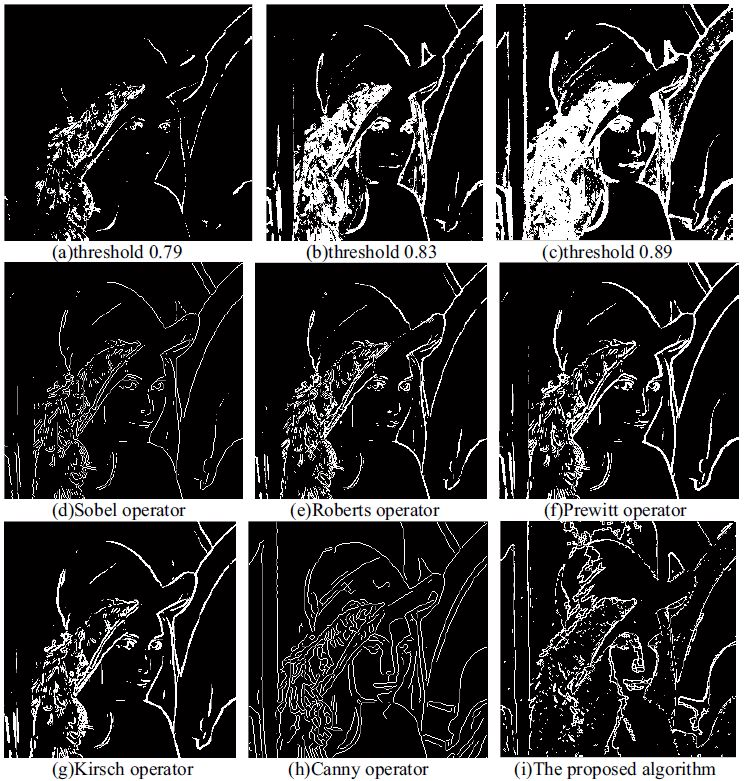
\includegraphics[resolution=300,scale=0.75]{/Example}
	\caption{}
	\label{fig:Sammenligning}
\end{figure}
\noindent

The article is step vise going through the mathematics of the improved algorithm and trying to explain how the step works. A test of the algorithm is conducted and some of the results from the steps are shown in \autoref{fig:Test}. The step vise changes seen at \autoref{fig:Test} is also therefore the also the goal for this mini project.
\begin{figure}[H]
	\centering
	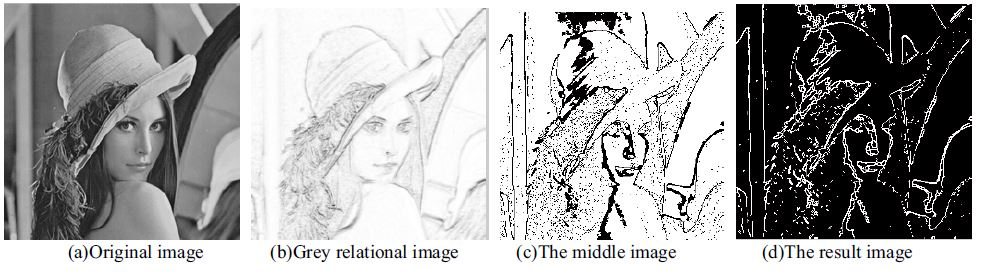
\includegraphics[resolution=300,scale=0.75]{/Test}
	\caption{}
	\label{fig:Test}
\end{figure}
\noindent
